This chapter outlines the theoretical and mathematical concepts of the high energy particle physics.
The Standard Model of particle physics (SM)~\cite{Salam:1968rm, Glashow:1961tr, Weinberg:1967tq, Herrero:1998eq, Cottingham:2007zz} is developed since the early 1970s and it has successfully explained almost all experimental results.
The SM is a well-tested and the most successful physics theory to describe the nature of the elementary particles and their interactions.
An overview of the SM is given in Sect.~\ref{sec:sm}.
After that, some of the open questions are mentioned in Sect.~\ref{sec:sm_bsm}.

%%%
%%%
%%%

\section{The Standard Model of Particle Physics}
\label{sec:sm}
The Standard Model of particle physics is known as the most accurate theory for describing the elementary particles and the interactions between them.
By combining the quantum mechanics and special relativity, the SM is a relativistic \textit{Quantum Field Theory} (QFT) based on a $SU(3)_{C} \otimes SU(2)_{L} \otimes U(1)_{Y}$ symmetry gauge group, where $C$ denotes colour, $L$ represents left chirality, and $Y$ stands for weak hypercharge, respectively.
The $SU(3)_{C}$ group is the basis for \textit{Quantum Chromodynamics} (QCD) which describes the strong interaction and the $SU(2)_{L} \otimes U(1)_{Y}$ group is the foundation of the electroweak interaction which unifies the electromagnetic and weak interactions.
Therefore, the SM Lagrangian is invariant under the local gauge transformation.
According to \textit{Noether's Theorem}~\cite{Noether:1918zz}, the invariance of an action of a physical system undergoes a symmetry transformation corresponding to a conservation law and vice versa. 
The gauge invariance of the SM Lagrangian corresponds to the conserved quantum numbers, or the charges, of each interaction.
The conserved charges are the three colour charge (red, blue, green) for the strong interaction, the third component of the weak isospin $I_{3}$ for the weak interaction, and the electric charge $Q$ for the electromagnetic interaction.

%%%
%%%
%%%

\subsection{Particle Content}
\label{subsec:sm_particle_content}
According to the SM, all matter around us is made of elementary particles called \textit{quarks} and \textit{leptons}.
The quarks and leptons are called fermions which have half integral spin $s=\frac{1}{2}$, hence the fermions follow the Pauli exclusion principle which says no two fermions have the same quantum state at the same time.
Each fermion has an anti-fermion with the equal mass but carries opposite electric charge, weak isospin and colour charge.
There are six quarks and six leptons, they are grouped into three pairs, or "\textit{generations}", ordered by their mass.
The lightest and most stable particles constitute the first generation and they are constituents of ordinary matter.
The heavier and less stable particles form the second and third generations and the heavier particles quickly decay to the next most stable particles.
The three generations of quarks are up ($u$) and down ($d$), charm ($c$) and strange ($s$), and top ($t$) and bottom ($b$) quarks.
The up-type quarks ($u, c, t$) carry $+\frac{2}{3}|e|$ charge and with isospin $+\frac{1}{2}$ while the down-type quarks ($d, s, b$) carry $-\frac{1}{3}|e|$ charge with isospin $-\frac{1}{2}$.
The quarks carry an additional colour charge of either red, green, or blue, and hence they only interact via the strong force.
Because the strong force holds quarks together, only non-integer charges of the quark combinations are experimentally allowed.
The quark combinations are called \textit{hadrons} which can be categorised into \textit{mesons} and \textit{baryons}.
The meson is composed by a quark and anti-quark pair ($q\bar{q}$) whereas the baryon is made up by three quarks ($qqq$ or $\bar{q}\bar{q}\bar{q}$).
Only colourless bound states of hadrons are allowed so the quark and anti-quark pair in a meson should contain colour and anti-colour and the three quarks in a baryon must carry different colours.
The leptons are colourless and are therefore participating in the weak and electromagnetic force only. 
They do not participate in the strong interaction.
The electron-type leptons ($e, \mu, \tau$) carry an elementary charge $|e|$ and their corresponding neutrinos ($\nu_{e}, \nu_{\mu}, \nu_{\tau}$) are neutral.
The neutrinos have very little mass and interact via weak force only.
A summarised table of the properties of quarks and leptons is given in Table~\ref{tab:sm_fermions}.

\begin{table}[htp]
    %\begin{center}
    \resizebox{\textwidth}{!}{% <------ Don't forget this %
        \begin{tabular}{cccccccc}
            \hline
            \hline
            Generation           & Fermion                 &              & particle          & electric charge $Q$ & weak isospin $I_{3}$ & colour charge $C$ & mass [{\GeV}]\\
            \hline
            \multirow{4}{*}{I}   & \multirow{2}{*}{Quark}  & $u$          & up quark          & $+\frac{2}{3}|e|$   & $+\frac{1}{2}$       & r,g,b             & 0.0023\\
                                 &                         & $d$          & down quark        & $-\frac{1}{3}|e|$   & $-\frac{1}{2}$       & r,g,b             & 0.0048\\
                                 & \multirow{2}{*}{Lepton} & $e$          & electron          & $-1|e|$             & $-\frac{1}{2}$       & -                 & 0.00051\\
                                 &                         & $\nu_{e}$    & electron neutrino & 0                   & $+\frac{1}{2}$       & -                 & $< 2 \times 10^{-9}$\\
            \hline
            \multirow{4}{*}{II}  & \multirow{2}{*}{Quark}  & $c$          & charm quark       & $+\frac{2}{3}|e|$   & $+\frac{1}{2}$       & r,g,b             & 1.275\\
                                 &                         & $s$          & strange quark     & $-\frac{1}{3}|e|$   & $-\frac{1}{2}$       & r,g,b             & 0.095\\
                                 & \multirow{2}{*}{Lepton} & $\mu$        & muon              & $-1|e|$             & $-\frac{1}{2}$       & -                 & 0.106\\
                                 &                         & $\nu_{\mu}$  & muon neutrino     & 0                   & $+\frac{1}{2}$       & -                 & $< 1.9 \times 10^{-7}$\\
            \hline
            \multirow{4}{*}{III} & \multirow{2}{*}{Quark}  & $t$          & top quark         & $+\frac{2}{3}|e|$   & $+\frac{1}{2}$       & r,g,b             & 173.2\\
                                 &                         & $b$          & bottom quark      & $-\frac{1}{3}|e|$   & $-\frac{1}{2}$       & r,g,b             & 4.18\\
                                 & \multirow{2}{*}{Lepton} & $\tau$       & tau               & $-1|e|$             & $-\frac{1}{2}$       & -                 & 1.777\\
                                 &                         & $\nu_{\tau}$ & tau neutrino      & 0                   & $+\frac{1}{2}$       & -                 & $< 1.82 \times 10^{-5}$\\
            \hline
            \hline
        \end{tabular}
    }
    %\end{center}
    \caption{The Standard Model fermions with charges and masses~\cite{Patrignani:2016xqp}.}
    \label{tab:sm_fermions}
\end{table}%

%\begin{figure}[htbp]
%   \begin{center}
%       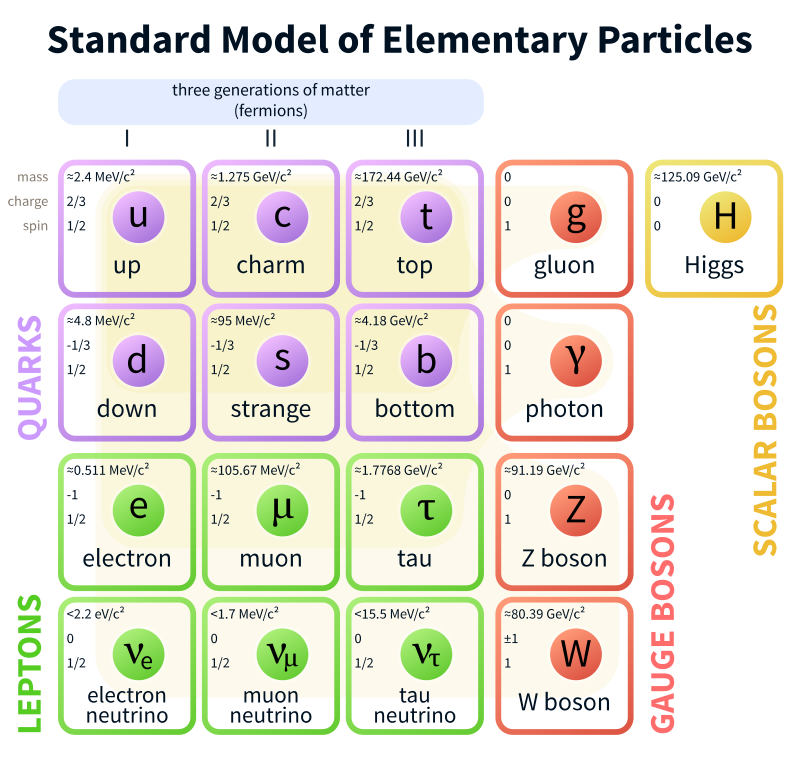
\includegraphics[scale=0.3]{800px-Standard_Model_of_Elementary_Particles.png}
%       \caption{default.
%       https://en.wikipedia.org/wiki/Standard_Model}
%       \label{fig:sm_particles}
%   \end{center}
%\end{figure}

There are four fundamental forces in the universe: the strong force, the weak force, the electromagnetic force, and the gravitational force.
The first three forces are described in the SM, however, the gravitational force could not yet be included in the SM.
Because the effect of the gravitational force is very weak and can be negligible, the SM works well without considering the gravitational force.
Each force has a force-carrier particle called gauge boson and there is a quantum number associate to it.
The gauge bosons of the strong force are eight massless \textit{gluons}, $g$, which associate to colour charge $C$.
The gauge bosons of the weak force are $W^{\pm}$ and $Z^{0}$ bosons which associate to weak isospin $I_{3}$.
The gauge boson of the electromagnetic force is massless \textit{photon}, $\gamma$, which associates to electric charge $Q$.
Although the gluon and photon are massless particles, the $W^{\pm}$ and $Z^{0}$ bosons are massive.
The mass of the $W^{\pm}$ and $Z^{0}$ bosons are $m_{W}=80.385 \pm 0.015$~{\GeV} and $m_{Z}=91.1876 \pm 0.0021$~{\GeV}~\cite{Patrignani:2016xqp}, respectively.
Table~\ref{tab:sm_fundamental_forces} shows the four fundamental forces, the relative strength and range together with the theories and the mediators.

\begin{table}[htp]
    %\begin{center}
    \resizebox{\textwidth}{!}{% <------ Don't forget this %
        \begin{tabular}{cccccc}
            \hline
            \hline
            Force           & Rel. Strength & Range [m]  & Theory             & Mediator                     & Mass [{\GeV}]\\
            \hline
            Strong          & $10$          & $10^{-15}$ & Chromodynamics     & Gluon                        & 0\\
            Weak            & $10^{-13}$    & $10^{-18}$ & Flavourdynamics    & $W^{\pm}$ and $Z^{0}$ bosons & 80.4/91.2\\
            Electromagnetic & $10^{-2}$     & $\infty$   & Electrodynamics    & Photon                       & 0\\
            \hline
            Gravitational   & $10^{-42}$    & $\infty$   & General relativity & Graviton                     & -\\
            \hline
            \hline
        \end{tabular}
    }
    %\end{center}
    \caption{The four fundamental forces with the relative strength, interaction range, describing theory, and the mediator with its mass.
    The gravitational force is not a part of the SM and the graviton is a theoretical particle.}
    \label{tab:sm_fundamental_forces}
\end{table}%

%%%
%%%
%%%

\subsection{Local Gauge Theory}
\label{subsec:sm_gauge_theory}
The Lagrangian density of the SM for the free fields\footnote{This is the Lagrangian density of QED. The three terms are fermion kinematic term, photon kinematic term, and interaction, respectively.} listed in the Eq.~(\ref{eq:sm_lagrangian}) is invariant under local gauge transformation\footnote{In Dirac representation, the four contravariant gamma matrices are $\gamma^{0} = \left(\begin{matrix}1 & 0 & 0 & 0\\0 & 1 & 0 & 0\\0 & 0 & -1 & 0\\0 & 0 & 0 & -1\end{matrix}\right)$, $\gamma^{1} = \left(\begin{matrix}0 & 0 & 0 & 1\\0 & 0 & 1 & 0\\0 & -1 & 0 & 0\\-1 & 0 & 0 & 0\end{matrix}\right)$, $\gamma^{2} = \left(\begin{matrix}0 & 0 & 0 & -i\\0 & 0 & i & 0\\0 & i & 0 & 0\\-i & 0 & 0 & 0\end{matrix}\right)$, $\gamma^{3} = \left(\begin{matrix}0 & 0 & 1 & 0\\0 & 0 & 0 & -1\\-1 & 0 & 0 & 0\\0 & 1 & 0 & 0\end{matrix}\right)$}
%
\begin{equation}
    \mathcal{L} = \bar{\psi}(i\gamma^{\mu}\partial_{\mu} - m)\psi + e\bar{\psi}\gamma^{\mu}\psi\bm{A}_{\mu} - \frac{1}{4}\bm{F}_{\mu\nu}\bm{F}^{\mu\nu}
    \label{eq:sm_lagrangian}
\end{equation}
%
where $\bm{F}_{\mu\nu} = \partial_{\mu}\bm{A}_{\nu} - \partial_{\nu}\bm{A}_{\mu}$.
The local gauge transformation means the scalar field $\psi$ and the vector field $\bm{A}_{\mu}$ transform as
%
\begin{align}
    \psi(x) & \rightarrow \psi'(x) = e^{i\theta(x)}\psi(x)\\
    \bm{A}_{\mu}(x) & \rightarrow \bm{A}_{\mu}'(x) = \bm{A}_{\mu}(x) + \frac{1}{e}\partial_{\mu}\theta(x).
    \label{eq:sm_gauge_transformation}
\end{align}
%
By introducing the gauge term, i.e. the vector field, the interacting force can be obtained by calculating the derivatives of the \textit{Euler-Lagrange equations}.
The gauge field can be associated to particular spin one gauge bosons which mediate the force.
The number of the mediating gauge bosons is equal to the dimension of the symmetry group.
From the group theory, the dimension of an unitary group $U(n)$ is $n^{2}$ and the dimension of a special unitary group $SU(n)$ is $n^{2} - 1$.
Because the SM is based on a $SU(3)_{C} \otimes SU(2)_{L} \otimes U(1)_{Y}$ symmetry gauge group, the number of mediators are 8 for $SU(3)_{C}$, 3 for $SU(2)_{L}$, and 1 for $U(1)_{Y}$ corresponding to 8 gluons for the strong interaction, 3 gauge bosons ($W^{\pm}$ and $Z^{0}$) for weak interaction, and 1 photon for the electromagnetic interaction.


%%%
%%%
%%%

\subsection{Strong interaction}
\label{subsec:sm_strong_interaction}
The \textit{Quantum Chromodynamics} (QCD) is the theory to describe the strong interaction.
The gauge bosons are the eight massless gluons which carry three different colours (and anti-colours), red, green, and blue.
Quarks interact with gluons hence they also carry colour charge $C$ and can be represented in colour triplets
%
\begin{equation}
    \psi = 
    \left(
        \begin{matrix}
            & \psi_{r} & \\
            & \psi_{g} & \\
            & \psi_{b} &
        \end{matrix}
    \right).
    \label{eq:sm_quark_triplets}
\end{equation}
%
The QCD is based on the non-Abelian $SU(3)_{C}$ group which requires local gauge transformation
%
\begin{equation}
    \psi \rightarrow \psi' = e^{i g_{s} \alpha_{a}(x) T^{a}}\psi
    \label{eq:sm_qcd_gauge_transformation_1}
\end{equation}
%
where the $g_{s}$ is the strong coupling constant, $\alpha_{a}(x)$ are arbitrary functions of space-time, and $T^{a}$ are the generators of the non-Abelian $SU(3)_{C}$ group and the summation over $a$ with $a = 1, \dots, 8$ is implied.
The Lagrangian density is invariant under the local gauge transformation by introducing the new form of the gauge fields and the covariant derivative
%
\begin{align}
    \bm{G}_{\mu}^{a} & \rightarrow \bm{G}_{\mu}^{a} -  \partial_{\mu} \alpha^{a}(x) - g_{s} f_{abc} \alpha^{b}(x) \bm{G}_{\mu}^{c} \\
    \partial_{\mu} & \rightarrow D_{\mu} = \partial_{\mu} + i g_{s} T_{a} \bm{G}_{\mu}^{a}
    \label{eq:sm_qcd_gauge_transformation_2}
\end{align}
%
where $f_{abc}$ is the structure constant. 
The Lagrangian density of QCD is given by
%
\begin{equation}
    \mathcal{L}_{QCD} = \bar{\psi}(i \gamma^{\mu} \partial_{\mu} - m) \psi - g_{s} ( \bar{\psi} \gamma^{\mu} T_{a} \psi) \bm{G}_{\mu}^{a} - \frac{1}{4} \bm{G}_{\mu\nu}^{a} \bm{G}_{a}^{\mu\nu}
    \label{eq:sm_qcd_lagrangian}
\end{equation}
%
where the field strength tensor $\bm{G}_{\mu\nu}^{a} = \partial_{\mu} \bm{G}_{\nu}^{a} - \partial_{\nu} \bm{G}_{\mu}^{a} - g_{s} f_{abc} \bm{G}_{\mu}^{b} \bm{G}_{\nu}^{c}$ causing self-interactions between the gluons.
The strong force increases with distance between quarks, therefore, the quarks exist only as colourless compounds such as meson or baryon mentioned in Sect.~\ref{subsec:sm_particle_content}.
The production of a single quark is accompanied by the creation of an anti-quark from vacuum to form a quark and anti-quark pair as a colourless compound.
This is called \textit{hadronisation}.
The phenomena that confined quarks in the small interaction range is called \textit{confinement}.
But at small distance or high energy, the quarks can be considered as quasi-free particles.
This is referred to as \textit{asymptotic freedom}.

%%%
%%%
%%%

\subsection{Electroweak interaction}
\label{subsec:sm_ewk_interaction}
Fermi formulated the first weak interaction theory in 1933~\cite{Fermi:1934hr}, however, the theory only holds for energies less than 100~{\GeV}.
Glashow, Salam, and Weinberg (GSW) proposed a new model~\cite{Salam:1968rm, Weinberg:1967tq, Glashow:1961tr} which unifies electromagnetic and weak forces to become \textit{electroweak} (EW) force and this new \textit{GSW model} can apply to the energy greater than 100~{\GeV}.
The electroweak theory is based on $SU(2)_{L} \otimes U(1)_{Y}$ gauge symmetry where the subscripts $L$ denotes the left-handedness because only the left-handed fermions (and right-handed anti-fermions) and $Y$ denotes the weak hypercharge, a new quantum number, which relates to the electric charge $Q$ and the weak isospin $I_{3}$ by the \textit{Gell-Mann-Nishijima relation}~\cite{Nakano:1953zz, Gell-Mann:1956iqa}
%
\begin{equation}
    Y = 2(Q - I_{3}).
    \label{eq:sm_hypercharge}
\end{equation}
%
The left-handed and right-handed fermion field $\psi$ can be decomposed into two components
%
\begin{align}
    \psi & = P_{L}\psi + P_{R}\psi\\
         & = \psi_{L} + \psi_{R}
    \label{eq:sm_fermion_field_components}
\end{align}
%
where the projection operators $P_{L}$ and $P_{R}$ are defined as\footnote{$\gamma^{5}$ is the product of the four gamma matrices. $\gamma^{5} = i \gamma^{0} \gamma^{1} \gamma^{2} \gamma^{3} = \left(\begin{matrix}0 & 0 & 1 & 0\\0 & 0 & 0 & 1\\1 & 0 & 0 & 0\\0 & 1 & 0 & 0\end{matrix}\right)$}
%
\begin{align}
    P_{L} & = \frac{1}{2} (1 - \gamma^{5})\\
    P_{R} & = \frac{1}{2} (1 + \gamma^{5}).
    \label{eq:sm_projection_operators}
\end{align}
%
The projection operators satisfy $P_{L}P_{R} = 0$ and $P_{L} + P_{R} = 1$.
Experimental observations show the right-handed neutrinos don't participate in all the interactions described in the SM so the $\psi_{R}$ is a singlet and $I_{3} = 0$\footnote{The left-handed fermion state $\psi_{L}$ is a doublet.}.
The local gauge transformations of the $SU(2)_{L} \otimes U(1)_{Y}$ are
%
\begin{align}
    \psi_{L} & \rightarrow \psi_{L}' = e^{i \alpha_{a}(x) T^{a}}e^{i \beta(x) Y} \psi_{L}\\
    \psi_{R} & \rightarrow \psi_{R}' = e^{i \beta(x) Y} \psi_{R}
    \label{eq:sm_local_gauge_transformations_ew_1}
\end{align}
%
where $T^{a} = \frac{\sigma^{a}}{2}$ are the generators of $SU(2)_{L}$ with Pauli matrix $\sigma^{a}$\footnote{The Pauli matrices are $\sigma_{1}=\left(\begin{matrix}0 & 1\\1 & 0\end{matrix}\right)$, $\sigma_{2}=\left(\begin{matrix}0 & -i\\i & 0\end{matrix}\right)$, and $\sigma_{3}=\left(\begin{matrix}1 & 0\\0 & -1\end{matrix}\right)$} and $Y$ is the generator of $U(1)_{Y}$.
The $\alpha_{a}(x)$ and $\beta(x)$ depend on the space-time.
The covariant derivative with respect to the $SU(2)_{L} \otimes U(1)_{Y}$ is
%
\begin{equation}
    D_{\mu} = \partial_{\mu} + i g_{W} T_{a} \bm{W}_{\mu}^{a} + i g_{Y} Y \bm{B}_{\mu}
    \label{eq:sm_derivative_ew}
\end{equation}
%
where $g_{W}$ and $g_{Y}$ are coupling constants and $\bm{W}_{\mu}^{a}$ ($a = 1, 2, 3$) and $\bm{B}_{\mu}$ are the gauge fields.
The gauge fields $\bm{W}_{\mu}^{a}$ and $\bm{B}_{\mu}$ transform under the $SU(2)_{L} \otimes U(1)_{Y}$ symmetry as
%
\begin{align}
    \bm{W}_{\mu}^{a} & \rightarrow \bm{W}_{\mu}^{a} - \frac{1}{g_{W}} \partial_{\mu} \alpha^{a}(x) - \epsilon^{abc} \alpha^{b}(x) \bm{W}_{\mu}^{c}\\
    \bm{B}_{\mu} & \rightarrow \bm{B}_{\mu} - \frac{1}{g_{Y}} \partial_{\mu} \beta(x)
    \label{eq:sm_local_gauge_transformations_ew_2}
\end{align}
%
where $\epsilon^{abc}$ is the Levi-Civita tensor.
The Lagrangian density of the electroweak is given by
%
\begin{equation}
    \mathcal{L}_{EW} = \bar{\psi}_{L} (i \gamma^{\mu} D_{\mu} - m) \psi_{L} + \bar{\psi}_{R} (i \gamma^{\mu} D_{\mu} - m) \psi_{R} - \frac{1}{4} \bm{W}_{\mu\nu}^{a} \bm{W}_{a}^{\mu\nu} - \frac{1}{4} \bm{B}_{\mu\nu} \bm{B}^{\mu\nu}
    \label{eq:sm_Lagrangian_ew}
\end{equation}
%
where $\bm{W}_{\mu\nu}^{a}$ and $\bm{B}_{\mu\nu}$ are the field strength tensors
%
\begin{align}
    \bm{W}_{\mu\nu}^{a} & = \partial_{\mu} \bm{W}_{\nu}^{a} - \partial_{\nu} \bm{W}_{\mu}^{a} - g_{W} \epsilon^{abc} \bm{W}_{\mu}^{b} \bm{W}_{\nu}^{c}\\
    \bm{B}_{\mu\nu} & = \partial_{\mu} \bm{B}_{\nu} - \partial_{\nu} \bm{B}_{\mu}
    \label{eq:sm_field_strangth_tensors}
\end{align}
%
and $\bar{\psi} \equiv \psi^{\dagger} \gamma^{0}$ is the adjoint spinor of $\psi$\footnote{$\psi^{\dagger}$ is the hermitian conjugate of $\psi$}.
Therefore, the mass eigenstates are the mixture of the gauge fields
%
\begin{align}
    \bm{W}_{\mu}^{\pm} & = \frac{1}{\sqrt{2}} (\bm{W}_{\mu}^{1} \mp i \bm{W}_{\mu}^{2})\\
    \left(\begin{matrix}\bm{A}_{\mu}\\\bm{Z}_{\mu}\end{matrix}\right) & = \left(\begin{matrix}\cos\theta_{W} & \sin\theta_{W}\\-\sin\theta_{W} & \cos\theta_{W} \end{matrix}\right) \left(\begin{matrix}\bm{B}_{\mu}\\\bm{W}_{\mu}^{3}\end{matrix}\right).
    \label{eq:sm_mass_eigenstates}
\end{align}
%
Thus, the mass eigenstates $\bm{A}_{\mu}$, $\bm{W}_{\mu}^{\pm}$, and $\bm{Z}_{\mu}$ are identified as the photon, $\gamma$, $W^{\pm}$ and $Z^{0}$ bosons experimentally.
The \textit{Weinberg weak mixing angle} $\theta_{W}$ is defined as
%
\begin{equation}
    \tan \theta_{W} = \frac{g_{Y}}{g_{W}}.
    \label{eq:sm_mixing_angle}
\end{equation}
%
The coupling constants $g_{W}$ and $g_{Y}$ are related to the electric charge by
%
\begin{equation}
    e = g_{W} \sin\theta_{W} = g_{Y} \cos\theta_{Y}.
    \label{eq:sm_coupling_constants}
\end{equation}
%
And the weak eigenstates of quark, $q'$, are the linear combinations of the mass eigenstates of quark, q, by the \textit{Cabbibo-Kobayashi-Maskawa} (CKM) matrix~\cite{Kobayashi:1973fv}
%
\begin{equation}
    \left(\begin{matrix}d'\\s'\\b'\end{matrix}\right) = \left(\begin{matrix}V_{ud} & V_{us} & V_{ub}\\V_{cd} & V_{cs} & V_{cb}\\V_{td} & V_{ts} &V_{tb}\end{matrix}\right) \left(\begin{matrix}d\\s\\b\end{matrix}\right).
    \label{eq:sm_CKM_matrix}
\end{equation}
%
The CKM matrix allows the quarks changing their flavour and generation as observed in the experiment.
Similarly, the \textit{Pontecorvo-Maki-Nakagawa-Sakata} (PMNS) matrix~\cite{Maki:1962mu} is responsible for the flavour changing of the neutrinos.

%%%
%%%
%%%

\subsubsection{Spontaneous symmetry breaking and Higgs mechanism}
\label{subsubsec:sm_Higgs_mechanism}
The gauge bosons of the weak interaction, $W^{\pm}$ and $Z^{0}$, are massive particles\footnote{$m_{W}=80.385 \pm 0.015$~{\GeV} and $m_{Z}=91.1876 \pm 0.0021$~{\GeV}}.
However, the existence of the mass terms violate the gauge invariance of the $\mathcal{L}_{EW}$.
In order to explain the mass of gauge bosons, the Englert-Brout-Higgs mechanism~\cite{Higgs:1966ev, Higgs:1964pj, Higgs:1964ia, Englert:1964et, Guralnik:1964eu} was proposed in 1964.
A new scalar complex $SU(2)_{L}$ doublet field $\Phi$ is introduced in the Higgs mechanism
%
\begin{equation}
    \Phi = \left(\begin{matrix}\Phi^{+}\\\Phi^{0}\end{matrix}\right) = \left(\begin{matrix}\Phi_{1} & i\Phi_{2}\\\Phi_{3} & i\Phi_{4}\end{matrix}\right)
    \label{eq:sm_higgs_doublet}
\end{equation}
%
with hypercharge $Y = 1$ and four degrees of freedom, $\Phi_{i}$, which are scalar fields and called the \textit{Goldstone modes}.
The Lagrangian density for this new field, Higgs field, is
%
\begin{equation}
    \mathcal{L}_{\Phi} = (D^{\mu}\Phi)^{\dagger}(D_{\mu}\Phi) - V(\Phi)
    \label{eq:sm_higgs_lagrangian}
\end{equation}
%
where the Higgs potential is defined as
%
\begin{equation}
    V(\Phi) = \mu^{2}|\Phi|^{2} + \lambda|\Phi|^{4}
    \label{eq:sm_higgs_potential}
\end{equation}
%
where $\mu$ and $\lambda$ are free parameters.
The Higgs potential is shown in Fig.~\ref{fig:sm_higgs_potential}.
The Higgs potential is the rotation $U(1)$ symmetry.
Choosing any of the points at the bottom of the Higgs potential breaks the symmetry spontaneously.
The \textit{spontaneously symmetry breaking} (SSB) means the Lagrangian keeps invariant under certain symmetry but no longer invariant at the ground state.

\begin{figure}[htbp]
    \begin{center}
        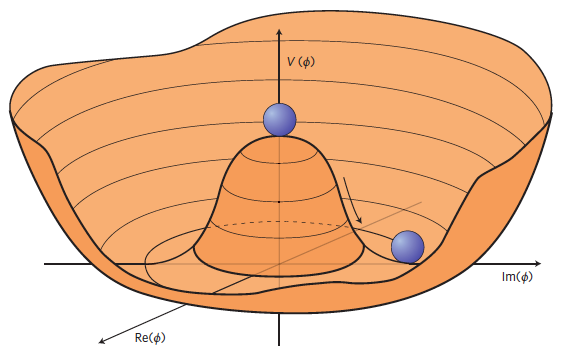
\includegraphics[scale=0.4]{higgspotential.png}
        \caption{An illustration of the Higgs potential which has the form of a ’Mexican hat’.
        The figure is taken from~\cite{Ellis:2013jnq}.}
        \label{fig:sm_higgs_potential}
    \end{center}
\end{figure}

Because the Higgs potential is invariant under $SU(2)_{L} \otimes U(1)_{Y}$, the parameters $\mu$ and $\lambda$ must satisfy $\mu^{2} < 0$ and $\lambda > 0$ resulting in a set of degenerate ground states where $\langle 0|\Phi|0 \rangle \neq 0$.
Among the degenerate ground states, the ground state is often chosen to have the form
%
\begin{equation}
    \Phi = \frac{1}{\sqrt{2}}\left(\begin{matrix}0\\v\end{matrix}\right)
    \label{eq:sm_ground_state}
\end{equation}
%
where $v = \sqrt{-\mu^{2}/\lambda}$ is the \textit{the vacuum expectation value} (VEV).
This particular choice of the ground state breaks the $SU(2)_{L} \otimes U(1)_{Y}$ symmetries spontaneously and  ensures the unbroken electromagnetic interaction under $U(1)_{EM}$ symmetry and photon being massless.
By introducing a massive particle, Higgs boson $H$, the Higgs field can be re-written as
%
\begin{equation}
    \Phi = \frac{1}{\sqrt{2}}\left(\begin{matrix}0\\v + H\end{matrix}\right)
    \label{eq:sm_ground_state_2}
\end{equation}
%
and the kinematic term of the Lagrangian density becomes
%
\begin{align}
    \mathcal{L}_{\Phi}^{\textrm{kinematic}} & = (D^{\mu}\Phi)^{\dagger}(D_{\mu}\Phi)\\
                                            & = \frac{1}{2}\partial_{\mu}H\partial^{\mu}H + (v + H)^{2}\Big\{\frac{g_{W}^{2}}{4} \bm{W}_{\mu}^{\dagger}\bm{W}^{\mu} + \frac{g_{W}^{2}}{8\cos^{2}\theta_{W}}\bm{Z}_{\mu}^{\dagger}\bm{Z}^{\mu}\Big\}
    \label{eq:sm_Lagrangian_kinematic_term}
\end{align}
%
and the Higgs potential is now
%
\begin{equation}
    V(\Phi) = -\frac{v^{2} \lambda}{2}(v+H)^{2} + \frac{\lambda}{4}(v+H)^{4}.
\end{equation}
%
Thus the masses of the $W^{\pm}$ and $Z^{0}$ are obtained by the interaction between the gauge bosons and Higgs boson.
The masses are defined as
%
\begin{equation}
    m_{H} = v\sqrt{2\lambda}, \quad m_{W} = \frac{v}{2}g_{W}, \quad m_{Z} = \frac{v}{2}\sqrt{g_{W}^{2} + g_{Y}^{2}}, \quad m_{\gamma} = 0.
\end{equation}
%
However, the masses of fermions are obtained by the \textit{Yukawa interaction}
%
\begin{equation}
    \mathcal{L}_{\textrm{Yukawa}} = y_{f} \bar{L}_{L} \Phi f_{R} + y_{f} \bar{Q}_{L} \Phi f_{R} + \textrm{h.c.}
\end{equation}
%
where the $y_{f}$ is \textit{Yukawa coupling}, $f$ stands for \{$\ell^{i}$, $u^{i}$, $d'^{i}$\} and h.c. represents the hermitian conjugate, respectively.
The $\bar{L}_{L}$ and $\bar{Q}_{L}$ are the left-handed lepton and quark doublet and $f_{R}$ is the lepton or quark singlet.
The mass of fermion is defined as
%
\begin{equation}
    m_{f} = \frac{v}{\sqrt{2}}y_{f}
\end{equation}
%
where $y_{f}$ is a free parameter which causes the fermion mass not predictable.
Finally, the non-zero VEV, $v$, can be related to \textit{Fermi constant}, $G_{F}$, by
%
\begin{equation}
    v = \frac{1}{\sqrt{\sqrt{2} G_{F}}} \approx 246 \textrm{~{GeV}}.
\end{equation}
%

%%%
%%%
%%%

\subsection{The discovery of Higgs boson}
A lot of the SM predictions are successfully confirmed by the experimental observations besides the existence of the theoretical Higgs boson. 
The search of the Higgs boson has become a major goal of the experimental particle physicists.
A Higgs-like resonance was discovered and announced on July 4th 2012 by the ATLAS\footnote{A Toroidal LHC ApparatuS} and CMS\footnote{Compact Muon Solenoid} collaborations~\cite{Aad:2012tfa, Chatrchyan:2012xdj}.
By combining the data with integrated luminosities of 4.8~{\ifb} collected at $\sqrt{s} = 7$~{\TeV} in 2011 and 5.8~{\ifb} at $\sqrt{s}=8$~{\TeV} in 2012, the ATLAS experiment measured the mass of the Higgs boson to be $126.0 \pm 0.4$ (stat.) $\pm 0.4$ (syst.)~{\GeV} with significance of 5.9$\sigma$ corresponding to a background fluctuation probability of $1.7 \times 10^{-9}$~\cite{Aad:2012tfa}.
In the meantime, the CMS experiment announced the mass of the Higgs boson to be $125.3 \pm 0.4$ (stat) $\pm 0.5$ (syst.)~{\GeV} with significance 5.0$\sigma$ using integrated luminosities of up to 5.1~{\ifb} at 7 TeV and 5.3~{\ifb} at 8 TeV~\cite{Chatrchyan:2012xdj}. 
The $H \rightarrow ZZ^{(*)} \rightarrow 4\ell$, $H \rightarrow \gamma \gamma$, and $H \rightarrow WW^{(*)} \rightarrow e\nu\mu\nu$ channels were studied by the ATLAS collaboration and the $H \rightarrow \gamma \gamma, ZZ, W^{+}W^{-}, \tau^{+}\tau^{-}$, and $b\bar{b}$ channels were studied by the CMS collaboration.
In the Fig.~\ref{fig:sm_discovery_of_Higgs} shows the local $p$-value as a function of the Higgs mass for ATLAS and CMS results, respectively.

\begin{figure}[htbp]
    \begin{center}
        \begin{subfigure}[b]{0.48\textwidth}
            \begin{center}
                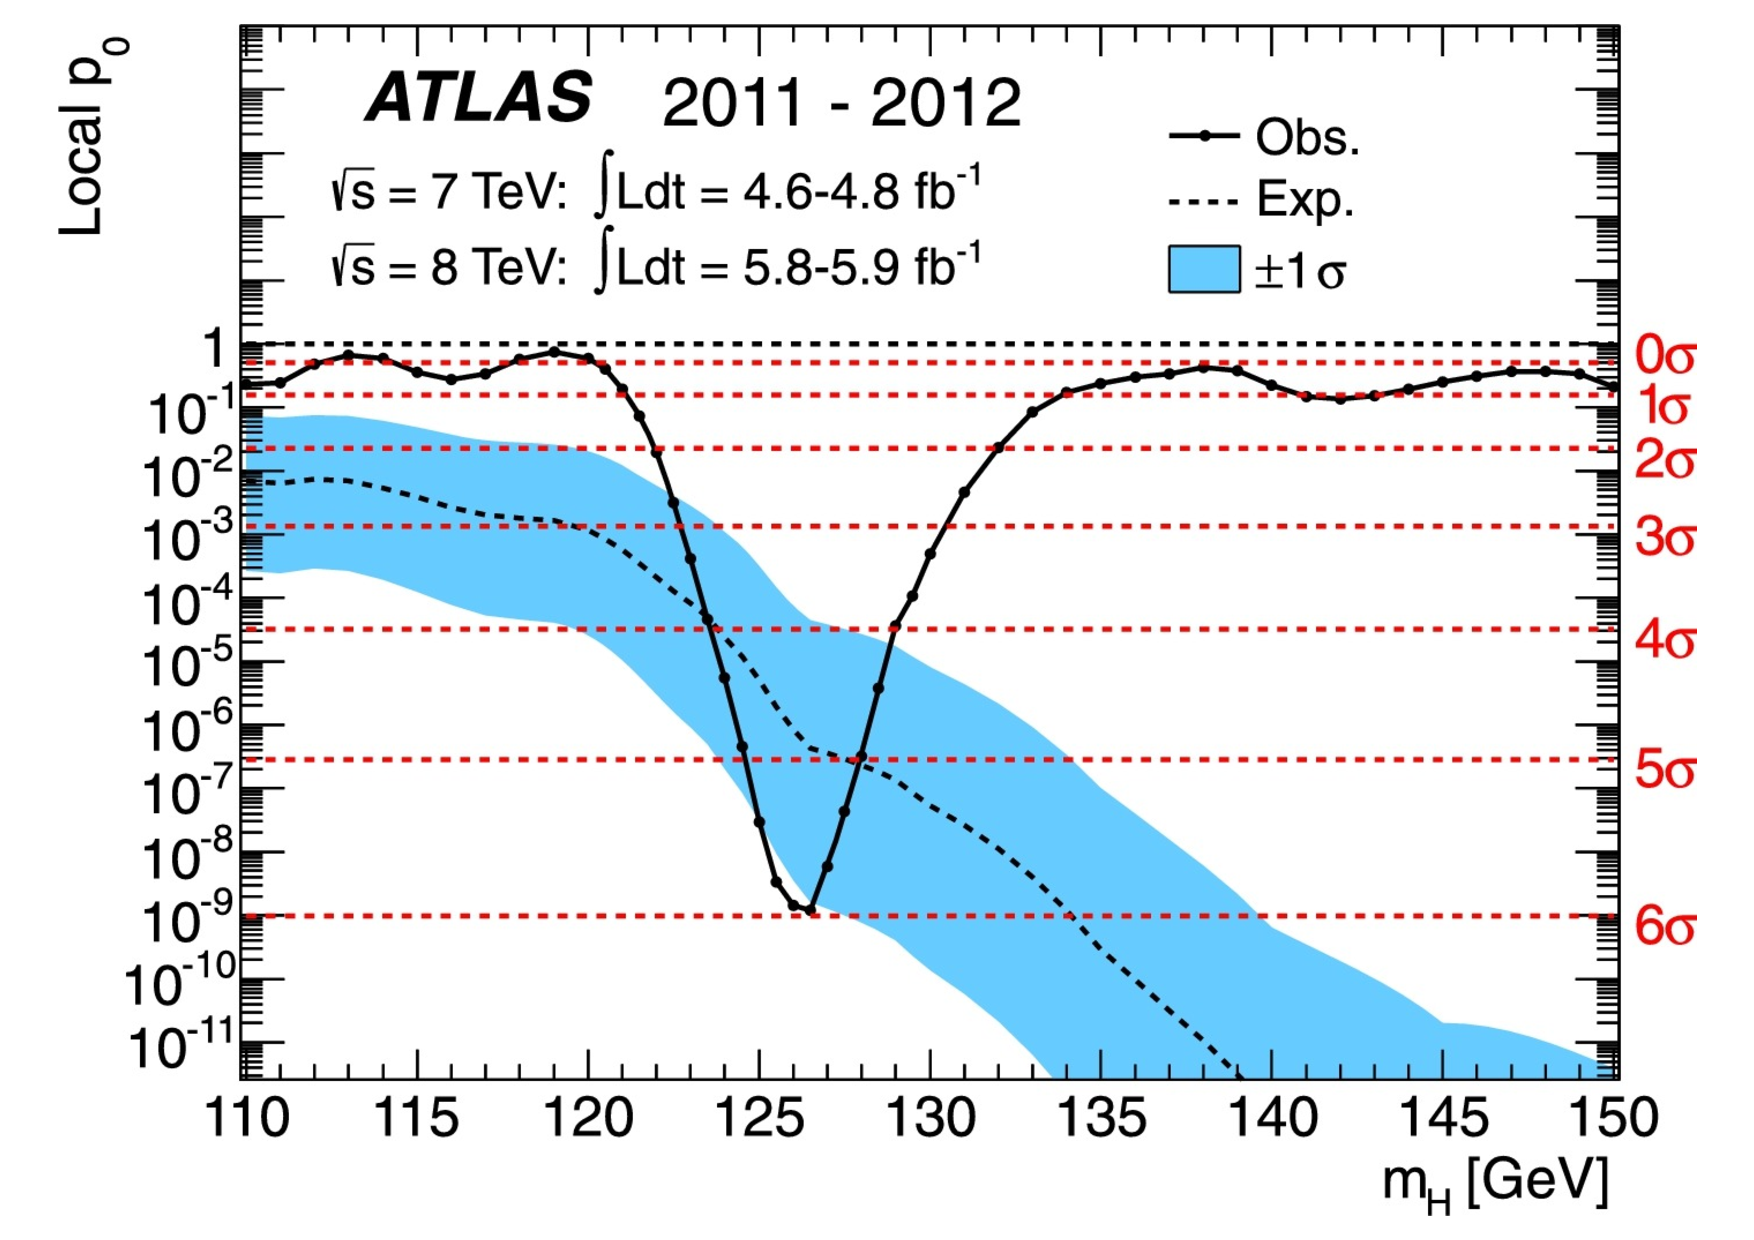
\includegraphics[scale=0.25]{1-s2_0-S037026931200857X-gr009_lrg.pdf}
                \caption{ATLAS results}
            \end{center}
        \end{subfigure}%
        \begin{subfigure}[b]{0.48\textwidth}
            \begin{center}
                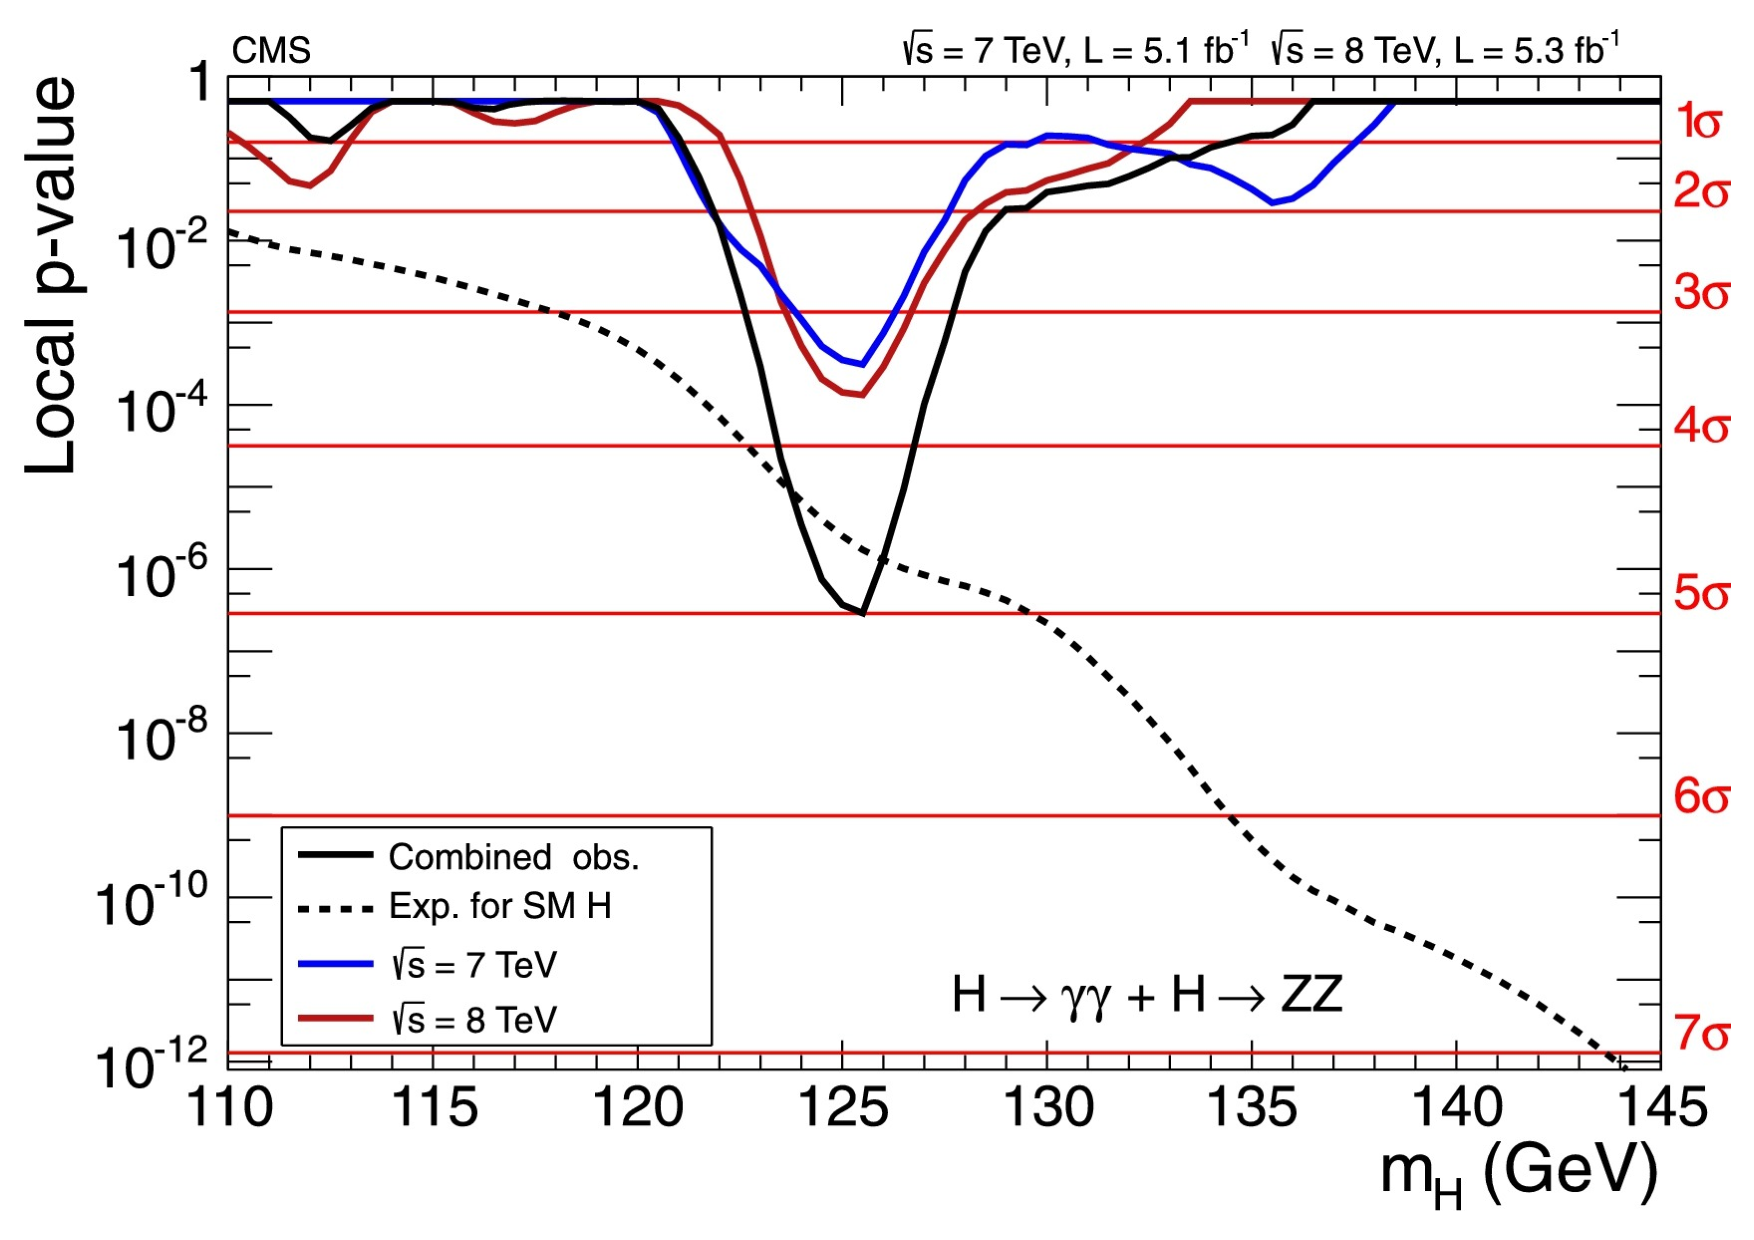
\includegraphics[scale=0.25]{1-s2_0-S0370269312008581-gr016_lrg.pdf}
                \caption{CMS results}
            \end{center}
        \end{subfigure}
    \end{center}
    \caption{The observed local $p$-value as a function of \mH for the ATLAS~\cite{Aad:2012tfa} and CMS~\cite{Chatrchyan:2012xdj} experiment, respectively.
    The dashed line shows the expected local $p_{0}$ for a SM Higgs boson.
    The horizontal lines denotes the $p$-values corresponding to significances of 1 to 6$\sigma$.}
    \label{fig:sm_discovery_of_Higgs}
\end{figure}

%%%
%%%
%%%

\section{Beyond the Standard Model}
\label{sec:sm_bsm}
Although the SM is an incredible successful theory for explaining the phenomenon in the particle physics, it leaves some questions which can no be answered.
Some of the unanswered questions are introduced in the rest part of this section.

%%%
%%%
%%%

\subsection{Hierarchy problem}
\label{subsec:sm_hierarchy_problem}
The weakest force in the SM is the weak force but the strength of the weak force is $10^{24}$ times as strong as gravitational force which doesn't incorporate into the SM.
The large discrepancy between the weak force and the gravitational force is called the hierarchy problem~\cite{Martin:1997ns, Chankowski:1998za, maarten_brak}.
The classical potential of the SM Higgs field $\Phi$ is
%
\begin{equation}
    V(\Phi) = \mu^{2} |\Phi|^2 + \lambda |\Phi|^4.
\end{equation}
%
Since the SM requires the VEV for $\Phi$, $\langle \Phi \rangle$, at the minimum of the potential non-vanishing, this only satisfied if $\mu^{2} < 0$ and $\lambda > 0$.
However, the parameter $\mu^{2}$ receives enormous radiative corrections causing it ultraviolet divergent as shown in Eq.~(\ref{eq:sm_mu2_correction}).
%
\begin{equation}
    \mu^{2} = \mu_{bare}^{2} - \frac{|\lambda_{f}|^{2}}{8\pi}\Lambda_{UV}^{2} + \mathcal{O}(\Lambda_{UV}^{2})
    \label{eq:sm_mu2_correction}
\end{equation}
%
where $\mu_{bare}$ is the Higgs mass, $- \frac{|\lambda_{f}|^{2}}{8\pi}\Lambda_{UV}^{2}$ is the one-loop correction, and $\Lambda_{UV}$ is an ultraviolet momentum cutoff which is valid up to the Plank scale $10^{19}$~{\GeV}.
The electroweak gauge bosons $W^{\pm}$ and $Z^{0}$ obtain their finite masses from $\langle \Phi \rangle$ so the $\mu^{2}$ cannot be divergent.
There must some unknown mechanism to protect from divergence.

%%%
%%%
%%%

\subsection{Dark matter and dark energy}
\label{subsec:sm_dm}
The matters we know today compose of only 5\%~\cite{Bennett:2012zja, Ade:2013sjv} of the content of the universe and the remaining part is something we don't know.
This unknown matter is called \textit{Dark Matter} (DM)~\cite{Bertone:2004pz} which makes up about 27\% of the universe and the rest 68\% are called \textit{Dark Energy} (DE)~\cite{Bennett:2012zja, Ade:2013sjv}.
Because DM interacts weakly and doesn't interact with the electromagnetic force, it doesn't absorb, emit, or reflect light causing it hard to detect directly. 
The name DM comes from it is invisible.
Dark energy distributes evenly in both space and time throughout the universe so it doesn't dilute when the universe expands.
The observed scientific data hints the presence of DE is necessary to explain the accelerated expansion of the universe.

%%%
%%%
%%%

\subsection{Grand Unification}
\label{subsec:sm_grand_unification}

\begin{figure}[tbp]
    \begin{center}
        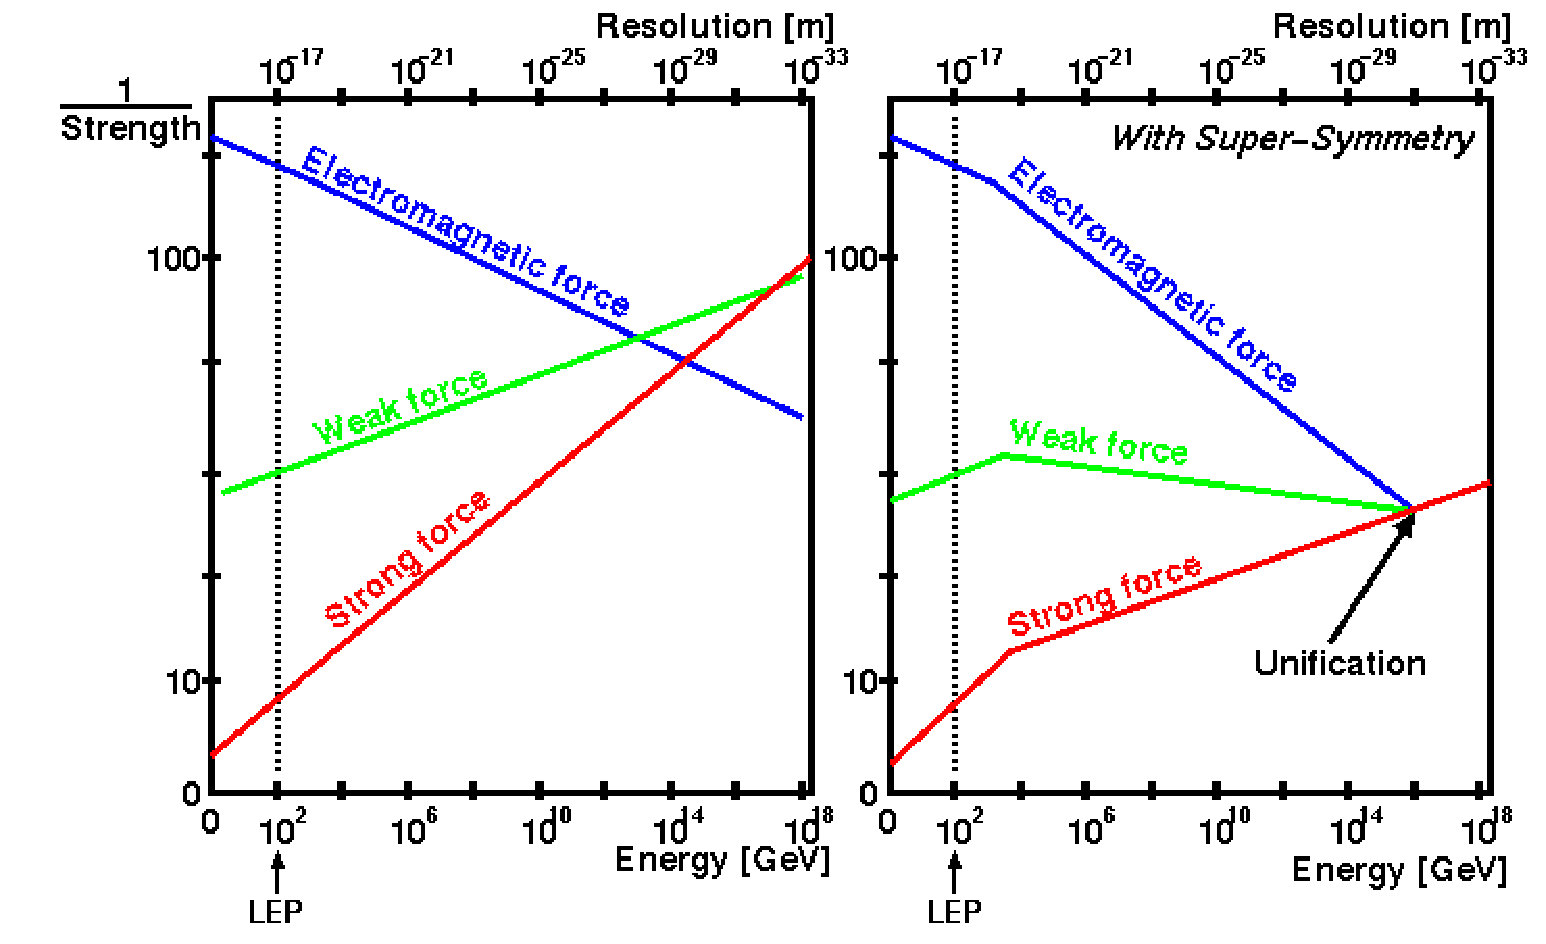
\includegraphics[scale=0.46]{running_coupling.pdf}
        \caption{The measured running coupling constants in the SM (left) and prediction in the GUT (right).
        The three lines show the inverse value of the coupling constant for the three fundamental forces.
        This figure is taken from~\cite{Ur0ol}.}
        \label{fig:sm_coulping_constants}
    \end{center}
\end{figure}

Maxwell unified the electricity and magnetism into electromagnetism in the 1860s.
About a century later, physicists successfully developed theory of electroweak which links the electromagnetism and the weak force.
Because of the triumph of electroweak theory, theorists raise the question of the possibility to unify all forces.
The \textit{Grand Unified Theory} (GUT)~\cite{Ross:1985ai}, which tries to link three of the four known forces together, is developed in the mid-1970s by theorists
The GUT proposes that the electromagnetic force, weak force, and strong force unify to one force at the GUT scale, $\Lambda_{GUT} \approx 10^{16}$~{\GeV}.
So the three running coupling constants~\cite{Mohr:2015ccw} are expected to be converged at the GUT scale.
However, the current experiment results show the coupling constants still different as shown in Fig.~\ref{fig:sm_coulping_constants}.

%%%
%%%
%%%

\subsection{More questions}
\label{subsec:sm_more_questions}
There are some more interesting questions which we don't know the answers.
For example, we don't know the reason why there are 61 elementary particles and more than 20 arbitrary parameters in the SM.
Also, the SM doesn't explain why there are only three generations.
The amount of matter and anti-matter are equal at the beginning of the universe based on the prediction of the SM but the matter dominates in the currently universe which the SM couldn't answer the reason why.

In order to answer these questions, there are many theories being developed on the top of SM but none of them has been observed.
One of the most probable candidate for answering these question is supersymmetry which will be introduced in the next chapter.
